\documentclass[11pt]{article}
\usepackage{latexsym}
\usepackage{amsmath}
\usepackage{amssymb}
\usepackage{amsthm}
\usepackage{epsfig}
\usepackage[tight]{subfigure}

\usepackage{amsmath}

\DeclareMathOperator*{\minimize}{min}
\DeclareMathOperator*{\maximize}{max}

\usepackage{algorithm}
 %on linux you may need to run sudo apt-get install texlive-full to install algorithm.sys
\usepackage{algorithmic}

\usepackage{verbatim}

% added by yenchi
\usepackage[pagebackref=true,breaklinks=true,letterpaper=true,colorlinks,citecolor=blue,linkcolor=blue,bookmarks=false]{hyperref}

% For editing
\usepackage{color}
\definecolor{crimson}{rgb}{0.86, 0.08, 0.24}
\definecolor{gray}{rgb}{0.5,0.5,0.5}
\definecolor{green}{rgb}{0, 0.4, 0}
\definecolor{orange}{rgb}{1, 0.5, 0}
\definecolor{mahogany}{rgb}{0.75, 0.25, 0.0}
\definecolor{purple}{rgb}{0.6, 0, 0.6}
\definecolor{darkgreen}{rgb}{0, 0.4, 0}
\definecolor{frenchblue}{rgb}{0.0, 0.45, 0.73}
\definecolor{red}{rgb}{1,0,0}
\definecolor{yellow}{rgb}{1,1,0}
\definecolor{magenta}{rgb}{1,0,1}
\definecolor{pink}{rgb}{1,0.412,0.706}
\definecolor{newgreen}{rgb}{0, 0.6, 0.2}
\definecolor{blue}{rgb}{0, 0, 1}

\ifx \submission \undefined
% 	\newcommand{\yenchi}[1]{{\color{frenchblue}{#1}}}
	\newcommand{\todo}[1]{({\color{purple}{#1}})}
\else
% 	\newcommand{\yenchi}[1]{{#1}}
	\newcommand{\todo}[1]{{#1}}
\fi

% \newcommand{\norm}[1]{\|#1\|_2}
\newcommand{\norm}[1]{\left\lVert#1\right\rVert}
\newcommand{\dotproduct}[2]{\langle #1 \, ,  #2 \rangle\,}

\newcommand{\name}{Yen-Chi Cheng}
\newcommand{\andrewid}{yenchich}
\newcommand{\question}{\noindent\textbf{Question: }}
\newcommand{\answer}{\noindent\textbf{Answer: }}

\newcommand{\hatyt}{\hat{y}_t}
\newcommand{\yt}{y_t}


\newcommand{\Av}{\mathbf{A}}
\newcommand{\av}{\mathbf{a}}

\newcommand{\Bv}{\mathbf{B}}
\newcommand{\bv}{\mathbf{b}}

\newcommand{\Uv}{\mathbf{U}}
\newcommand{\uv}{\mathbf{u}}

\newcommand{\Pv}{\mathbf{P}}
\newcommand{\pv}{\mathbf{p}}

\newcommand{\Mv}{\mathbf{M}}
\newcommand{\mv}{\mathbf{m}}

\newcommand{\Wv}{\mathbf{W}}
\newcommand{\wv}{\mathbf{w}}

\newcommand{\Xv}{\mathbf{X}}
\newcommand{\xv}{\mathbf{x}}
% uncomment the following def for final draft
% \def \final {}
\ifx \final \undefined
    % \newcommand{\yenchi}[1]{{\color{frenchblue}{YC:#1}}}
    \newcommand{\yenchi}[1]{{\color{frenchblue}{#1}}}
	\newcommand{\haoming}[1]{{\color{orange}{#1}}}
	\newcommand{\todo}[1]{{\color{purple}{(#1)}}}
	\newcommand{\todorep}[2]{{\sout{#1}}~{\color{purple}{#2}}}
\else
	\newcommand{\yenchi}[1]{{#1}}
	\newcommand{\haoming}[1]{{#1}}
	\newcommand{\todo}[1]{{#1}}
	\newcommand{\todorep}[2]{{#2}}
\fi


\newcommand{\handout}[5]{
  \noindent
  \begin{center}
  \framebox{
    \vbox{
      \hbox to 5.78in { {#1} \hfill #2 }
      \vspace{4mm}
      \hbox to 5.78in { {\Large \hfill #5  \hfill} }
      \vspace{2mm}
      \hbox to 5.78in { {\em #3 \hfill #4} }
    }
  }
  \end{center}
  \vspace*{4mm}
}

\newcommand{\lecture}[5]{\handout{#1}{#2}{#3}{#4}{#5}}
\newcommand{\collision}[0]{\mathrm{collision}}
\newcommand{\nocollision}[0]{\overline{\collision}}

\newcommand*{\QED}{\hfill\ensuremath{\square}}

\newtheorem{theorem}{Theorem}
\newtheorem{corollary}[theorem]{Corollary}
\newtheorem{lemma}[theorem]{Lemma}
\newtheorem{observation}[theorem]{Observation}
\newtheorem{proposition}[theorem]{Proposition}
\newtheorem{definition}[theorem]{Definition}
\newtheorem{claim}[theorem]{Claim}
\newtheorem{fact}[theorem]{Fact}
\newtheorem{assumption}[theorem]{Assumption}
\newtheorem{note}[theorem]{Note}

% 1-inch margins, from fullpage.sty by H.Partl, Version 2, Dec. 15, 1988.
\topmargin 0pt
\advance \topmargin by -\headheight
\advance \topmargin by -\headsep
\textheight 8.9in
\oddsidemargin 0pt
\evensidemargin \oddsidemargin
\marginparwidth 0.5in
\textwidth 6.5in

\parindent 0in
\parskip 1.5ex
%\renewcommand{\baselinestretch}{1.25}

%%% DISCLAIMER: we reference some of the content from Spring 2020's scribe note: https://www.dropbox.com/sh/j92mhvfeukmuz2f/AABTdMvmDghIx98YTBW9XMI1a?dl=0&preview=Lecture_4_PWEA_RWMA__OLC_Perceptron.pdf
%%% Some other reference:
%   - https://en.wikipedia.org/wiki/Winnow_(algorithm)
%   - https://en.wikipedia.org/wiki/Perceptron

\begin{document}

\lecture{Statistical Techniques in Robotics (16-831, S21)}{Lecture \#05
  (Monday, February 15)}{Lecturer: Kris Kitani}{Scribes: Yen-Chi Cheng, Hao-Ming Fu}{Online Linear Classification (Perceptron, Winnow)}


\section{Review}
% \subsection{Weighted Majority Algorithm (WMA)}
\normalfont
In the last lectures, we relax the realizability assumption and covered the two algorithms: Weighted Majority Algorithm (WMA) and Randomized Weighted Majority Algorithm (RWMA).

The Weighted Majority Algorithm (WMA) learns a weight for each expert and use their weighted opinion to make predictions. Also, the weights are updated according to the performance of their corresponding experts. To be more precise, in each round, the weights of the experts who fail to provide correct advice are lowered by a factor $(1 - \eta)$. The algorithm is as follows:

\begin{algorithm}[H]
\caption{Weighted Majority Algorithm (WMA)}
\label{algo:wma}
\begin{algorithmic}[1]
\STATE $\pmb{w}^{(1)} \leftarrow \{w_n^{(1)}=1\}_{n=1}^N$ \hfill $\triangleright$ Weight initialization
\STATE $\eta\leq\frac{1}{2}$\hfill $\triangleright$ Penalty rate initialization
\FOR{$t=1,\;\cdots,\;T$}
\STATE \textsc{Receive} ($\pmb{x}^{(t)}\in\{-1, 1\}^N$) \hfill $\triangleright$ Receive expert predictions
\STATE $\hat{y}^{(t)} = \text{sign}\Big(\sum_{n=1}^Nx_n^{(t)}\cdot w_n^{(t)}\Big)\in\{-1, 1\}$ \hfill $\triangleright$ Make learner prediction
\STATE \textsc{Receive} ($y^{(t)}\in\{-1, 1\}$) \hfill $\triangleright$ Receive actual answer
\STATE $w_n^{(t+1)}\leftarrow w_n^{(t)}\big(1-\eta\cdot\pmb{1}[y^{(t)}\neq x_n^{(t)}]\big)$ \hfill $\triangleright$ Weight update
\ENDFOR
\end{algorithmic}
\end{algorithm}

The upper bound of mistakes made by WMA is as follows:

\begin{align*}
    M^{(t)}&\leq\frac{2\log N}{\eta} + 2m_n^{(t)}(1+\eta)\;\;\;\forall n
\end{align*}

Also, we derived the upper bound of the regret of WMA:

\begin{align}
    R(h_n) = M^{(T)} - m_n^{(T)} \leq m_n^{(T)} + 2\eta m_n^{(T)} + \frac{2\log N}{\eta}
\end{align}

By considering possible choices of $\eta$, we concluded that the average regret of WMA doesn't converge to zero over time and, thus, WMA is not a no-regret algorithm.

Then, we introduced Randomized Weighted Majority Algorithm (RWMA). The difference between RWMA and WMA is that RWMA samples a single expert to follow rather than using the weighted opinions of the experts. Specifically, the weights of the experts serve as the probability distribution of the sampling process. The algorithm is as follows.

\begin{algorithm}[H]
\caption{Randomized Weighted Majority Algorithm (RWMA)}
\label{algo:rwma}
\begin{algorithmic}[1]
\STATE $\textbf{w}^{(1)} \leftarrow \{w_n^{(1)}=1\}_{n=1}^N$ \hfill $\triangleright$ Weight initialization
\STATE $\eta\leq\frac{1}{2}$\hfill $\triangleright$ Penalty rate initialization
\FOR{$t=1,\;\cdots,\;T$}
\STATE \textsc{Receive} ($\textbf{x}^{(t)}\in\{-1, 1\}^N$) \hfill $\triangleright$ Receive experts predictions
\STATE $I\sim$ \textsc{Multinomial}($\textbf{w}^{(t)}/\Phi^{(t)}$), where $\Phi^{(t)}=\sum_{n=1}^Nw_n^{(t)}$
\STATE $\hat{y}^{(t)}=h_i(\textbf{x}^{(t)})$ \hfill $\triangleright$ Make learner prediction via sampling
\STATE \textsc{Receive} ($y^{(t)}\in\{-1, 1\}$) \hfill $\triangleright$ Receive actual answer
\STATE $w_n^{(t+1)}\leftarrow w_n^{(t)}\big(1-\eta\cdot\textbf{1}[y^{(t)}\neq h_n(\textbf{x})^{(t)}]\big)$ \hfill $\triangleright$ Weight update
\ENDFOR
\end{algorithmic}
\end{algorithm}

We calculated the upper bound of expected mistakes and obtained:

\begin{align*}
    \mathbb{E}[M^{(T)}]&\leq (1+\eta)m_n^{(T)} + \frac{\log N}{\eta}
\end{align*}

Following this, we derived the upper bound of expected regret of RWMA:

\begin{align}
    \mathbb{E}[R] = \mathbb{E}[M^{(T)}] - m_n^{(T)} \leq \eta m_n^{(T)} + \frac{\log N}{\eta} \label{eq:rwma_final}
\end{align}

With this, we noticed that if we set $\eta$ to $\frac{1}{\sqrt{T}}$, the average regret of RWMA converges to zero over time. Thus, RWMA is a no-regret algorithm.

%%%%%%

% \section{Summary for Lecture \#05}
\section{Online Linear Classification}
% \label{ssec:online_linear_cls}

Linear classification algorithms are usually allowed to make use of all available data altogether. On the other hand, in an online learning scenario, a learning algorithm has to consider the training samples one by one. Here we will include two online linear classification algorithms, the Perceptron algorithm and the Winnow algorithm. They are similar in many ways, while using different approaches to update the model parameters and assumes different assumptions. Online Linear Classification falls into the category of Online Learning Classification, and the comparison between PWEA could be seen below:

% 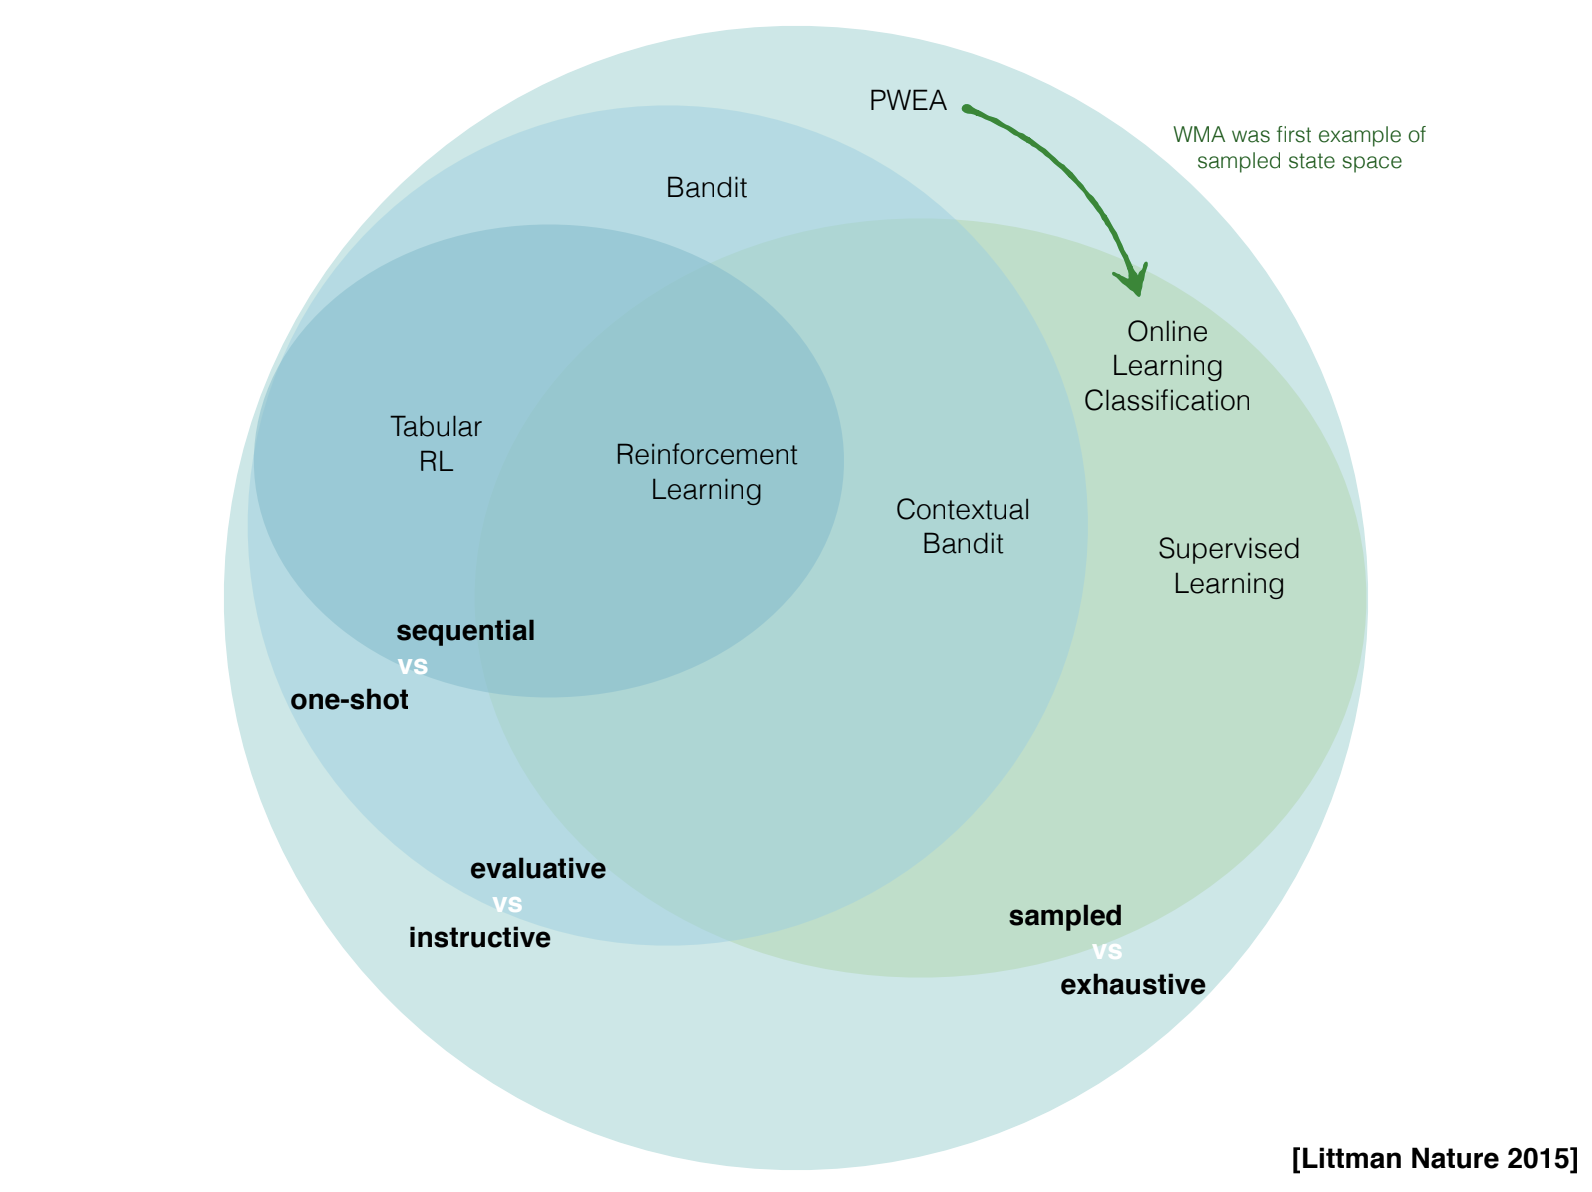
\includegraphics[width=.6\linewidth]{img/diagram.png}

\begin{figure}[H]
    \centering
    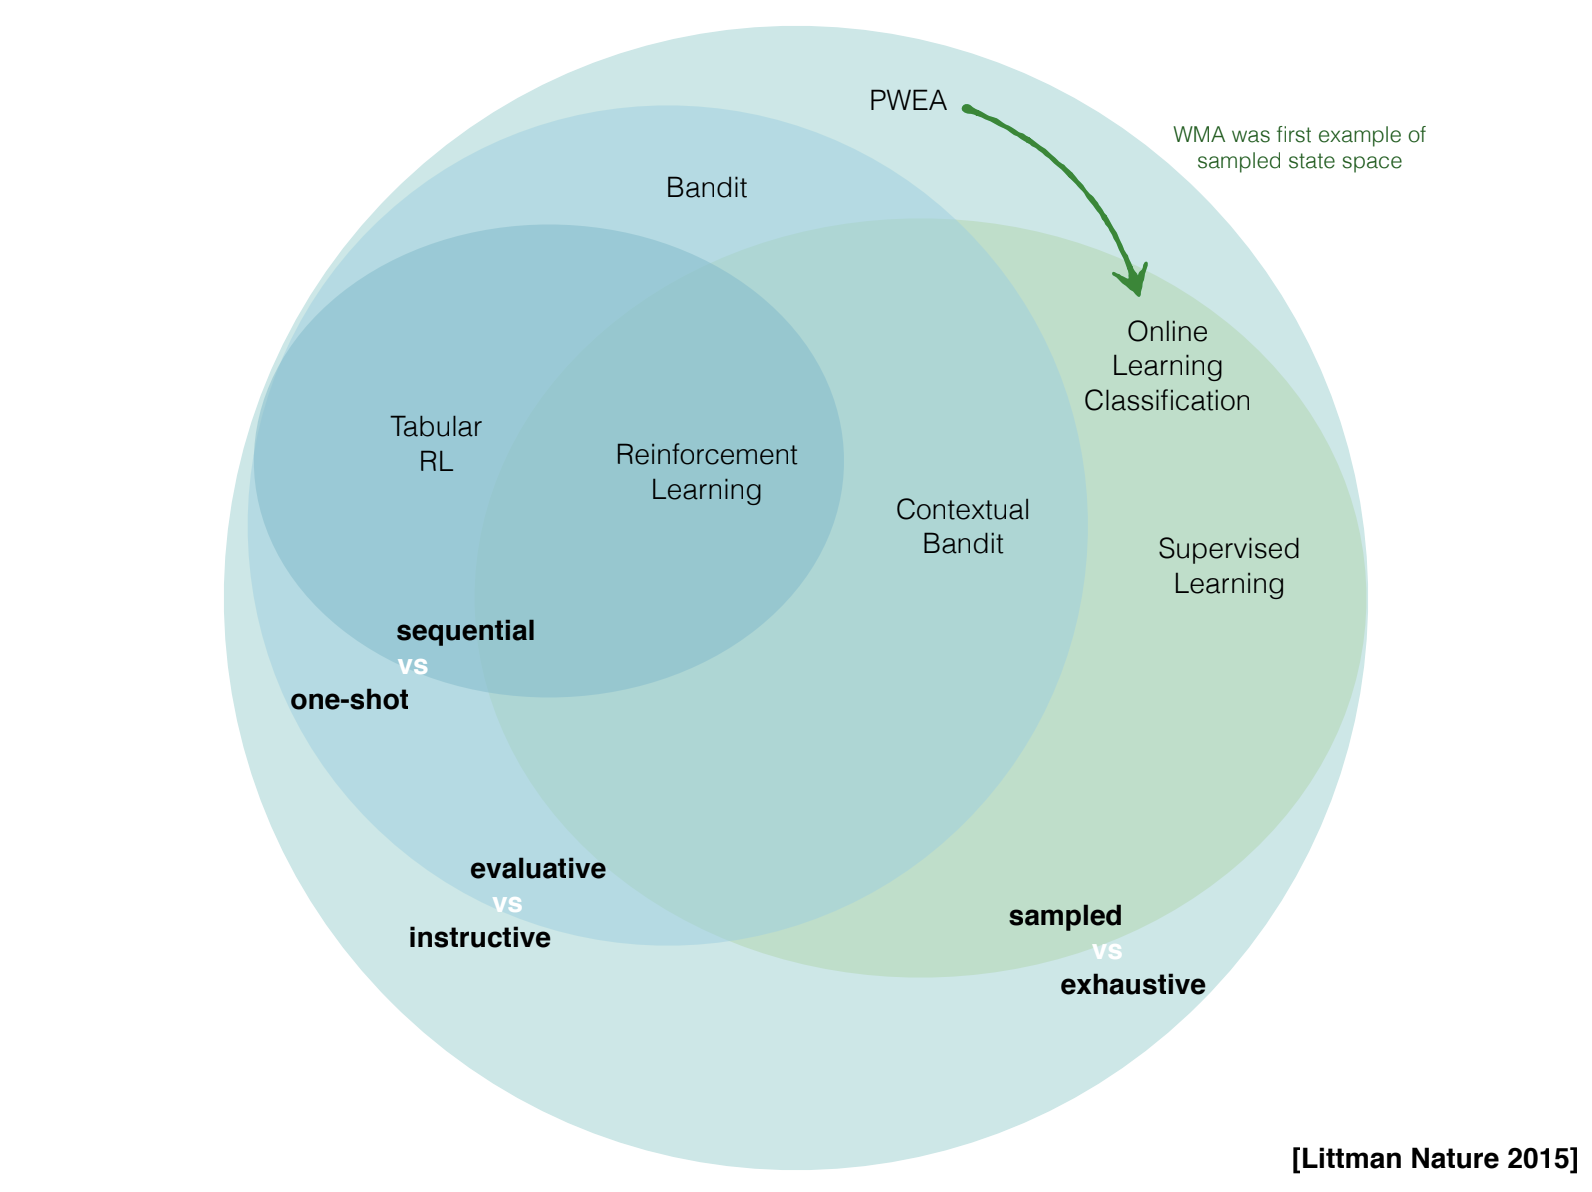
\includegraphics[width=.6\linewidth]{img/diagram.png}
    % \caption{Caption}
    % \label{fig:my_label}
\end{figure}


\section{Perceptron Algorithm}

\subsection{Overview}
\normalfont

The Perceptron Algorithm is an algorithm proposed by Rosenblatt~\cite{rosenblatt1958perceptron}. It can be used to learn a online linear classifier, and the algorithm is shown at Algorithm~\ref{algo:perceptron}. Intuitively, we could understand this algorithm as finding a ``hyperplane'' that separates the instance $\mathbf{x}^{(t)}$ in a high dimensional space $R^{N}$. The weight $w^{(t)}$ is the normal vector to that hyperplane, and will be updated with Eq. 6 at Algorithm~\ref{algo:perceptron} once it makes a mistake. Note that we assume the data is linearly separable. %($y^{t} = -1$ but is located at the plus-side of the hyperplane).

\begin{algorithm}[H]
\caption{Perceptron Algorithm}
\label{algo:perceptron}
\begin{algorithmic}[1]
\STATE $\pmb{w}^{(1)} \leftarrow \mathbf{0}$ \hfill $\triangleright$ Weight initialization
\FOR{$t=1,\;\cdots,\;T$}
\STATE \textsc{Receive} ($\pmb{x}^{(t)}\in \mathbb{R}^N$) \hfill $\triangleright$ Receive expert predictions
\STATE $\hat{y}^{(t)} = \text{sign}\Big( \dotproduct{ \pmb{w}^{(t)} }{\pmb{x}^{(t)} } \Big)$ \hfill $\triangleright$ Make learner prediction
\STATE \textsc{Receive} ($y^{(t)}\in\{-1, 1\}$) \hfill $\triangleright$ Receive actual answer
\STATE $\pmb{w}^{(t)}\leftarrow \pmb{w}^{(t-1)} + y^{(t)} \cdot \pmb{x}^{(t)} \cdot \pmb{1}[y^{(t)}\neq \hat{y}^{(t)}] $ \hfill $\triangleright$ Weight update
\ENDFOR
\end{algorithmic}
\end{algorithm}

The update value $y^{(t)} \cdot x^{(t)} \cdot\textbf{1}[y^{(t)}\neq \hat{y}^{(t)}]$ could either be positive or negative, as both $y^{(t)}$ or $x^{(t)}$ could be negative.

\subsection{Properties of the Perceptron Algorithm}
We discuss some of the properties regarding the Perceptron Algorithm.

\begin{enumerate}
    \item \textit{{\color{blue}{Is it fast?}}} \textbf{Yes.} The prediction is a dot product and a sign function, and the update rule only involves a dot product and a sum when it makes a mistake.
    \item \textit{{\color{blue}{Is it a Large Margin classifier?}}} \textbf{No}. It only looks at the sign of the dot product, so there is no notion of margin in the Perceptron Algorithm.
    \item \textit{{\color{blue}{Does it work on non-separable data?}}}  \textbf{No.} ``Non-separable'' means that we cannot find a linear decision boundary that perfectly separates the data. Therefore, it cannot work on non-separable data. However, when the data is linearly separable, the Perceptron Algorithm will make a finite number of mistakes~\cite{novikoff1963convergence}.
\end{enumerate}

\subsection{Mistake Bound}
We derive the mistake bound for the Perceptron Algorithm. Recall the 5-step strategy we used on previous algorithms: 1) define ``\textbf{potential}'' function, 2) \textbf{upper bound} the potential function, 3) \textbf{lower bound} the potential function, 4) combine bounds, 5) Algebra/approximation to get performance bound. Note that we do not derive the regret bound since we assume the linear separability.

\theorem{(Mistake bound of the Perceptron Algorithm) Let $M$ be the total mistakes made by the Perceptron Algorithm, $R=\underset{x}{\mathrm{max}} \norm{\pmb{x}^{(t)}}$ is the norm of the observations, and $\gamma = \underset{x}{\mathrm{min}} \, y_{t} \langle \pmb{w}^{*}\,,\pmb{x}^{(t)}\rangle$ is the margin of separability. Then $M$ is bounded by:
\label{theorm:perceptron}}{}

\begin{align}
    M \leq \frac{R^{2}}{\gamma^{2}}
\end{align}

\proof{\textbf{Upper bound of the potential function.} We start by defining the potential function:
\begin{align}
  \Phi^{(t)} = \norm{\pmb{w} ^ {(t)}}^{2} = \sum_{n=1} {(w_n^{(t)})}^{2}\label{eq:perceptron_potential}
\end{align}
with some derivation, we have
\begin{align}
  \Phi^{(t)} &= \norm{ \pmb{w} ^ {(t-1)} + y^{t}\pmb{x}^{(t)}}^{2} = \sum_{n=1} {(w_n^{(t)})}^{2}\, , \\
             &= \norm{ \pmb{w} ^ {(t-1)} }^{2} + \norm{ \pmb{x} }^{2} + 2 y^{(t)} \langle \pmb{w}^{(t-1)} \, , \pmb{x} ^{t} \rangle\, .
\end{align}  
since $2 y^{(t)} \langle \pmb{w}^{(t-1)} \, , \pmb{x} ^{t} \rangle\,$ must be negative because the learner makes a mistake at time $t$. Hence,
\begin{align}
  \Phi^{(t)} &= \norm{ \pmb{w} ^ {(t-1)} }^{2} + \norm{ \pmb{x} }^{2} + 2 y^{(t)} \langle \pmb{w}^{(t-1)} \, , \pmb{x} ^{t} \rangle\, , \\
             &\le \norm{ \pmb{w} ^ {(t-1)} }^{2} + \norm{ \pmb{x} }^{2} \,, \\
             &\le  \norm{ \pmb{w} ^ {(t-1)} }^{2} + R^2 \,. \label{eq:potential_upper1}
\end{align} 
Equation~\ref{eq:potential_upper1} is obtained by replacing $\norm{ \pmb{x} }$ with $R=\underset{x}{\mathrm{max}} \norm{\pmb{x}^{(t)}}$. \\
%
And the upper bound could be obtained using induction. Starting from the base case,
\begin{align}
  \Phi^{(1)} &\le  \norm{ \pmb{w} ^ {(0)} }^{2} + R^2 \,, \,\,\,\,\,\,\,\,\,\,\,\,\,\,\,\,\,\,\, \text{(1 mistakes)} \nonumber \\
  \Phi^{(2)} &\le  \norm{ \pmb{w} ^ {(0)} }^{2} + 2R^2 \,, \,\,\,\,\,\,\,\,\,\,\,\,\,\,\,\, \text{(2 mistakes)}      \nonumber \\
    &\vdots \nonumber\\
  \Phi^{(T)} &\le  \norm{ \pmb{w} ^ {(0)} }^{2} + M^{(T)}R^2 \, , \,\,\,\,\, \text{(M mistakes)}                     \nonumber \\
  \Phi^{(T)} &\le  M^{(T)}R^2 \label{eq:potential_upper2}
\end{align}
So we obtain the \textbf{upper bound} for the potential function. \\ \\
%
\textbf{Lower bound of the potential function.} The lower bound is a little tricky. We adopt an strategy to first define an intermediate potential $\dotproduct{\pmb{w}^{*}}{\pmb{w}^{(t)}}$, where $\pmb{w}^{*}$ is the perfect classifier and is a unit vector, and then upper bound and lower bound this dot product to derive the lower bound for $\Phi^{(t)}$. We start from the upper bound for this dot product. Observe that, 
\begin{align}
\frac{\pmb{w}}{\norm{ \pmb{w} }} = \underset{\pmb{w}^{\prime}}{\mathrm{argmax}} \dotproduct{ \pmb{w}^{\prime} }{ \pmb{w} }
\end{align}
since the dot product is largest when two vectors are oriented in the same direction. Note that $\pmb{w}^*$ is a unit vector, the dot product is maximized when:
\begin{align}
\dotproduct{ \pmb{w}^{*} }{ \pmb{w}^{(T)} } \le \dotproduct{\frac{ \pmb{w}^{(T)} }{ \norm{\pmb{w}^{(T)}  } }}{ \pmb{w}^{(T)} } = \frac{ \norm{ \pmb{w}^{(T)} }^{2} }{ \norm{ \pmb{w}^{(T)} } } = \norm{ \pmb{w}^{(T)} } \, . \label{eq:inter_potential_upper}
\end{align}
Therefore the upper bound is $\dotproduct{ \pmb{w}^{*} }{ \pmb{w}^{(T)} } \le \norm{ \pmb{w}^{(T)} }$. We proceed the proof by deriving the lower bound for $\dotproduct{ \pmb{w}^{*} }{ \pmb{w}^{(t)} }$. By applying the update rule to $ \pmb{w}^{(t)} $,
\begin{align}
    \dotproduct{ \pmb{w}^{*} }{ \pmb{w}^{(t)} } = \dotproduct{ \pmb{w}^{*} }{ \pmb{w}^{(t-1)} } + y^{(t)} \dotproduct{\pmb{w}^{*}}{\pmb{x}^{(t)}}\, . \label{eq:12}
\end{align}
note that $y^{(t)} \dotproduct{\pmb{w}^{*}}{\pmb{x}^{(t)}}$ is always positive because $\pmb{w}^{*}$ is the perfect classifier. Plug in $\gamma = \underset{x}{\mathrm{min}} \, y_{t} \dotproduct{\pmb{w}^{*}}{\pmb{x}^{(t)}}$,
\begin{align}
    \dotproduct{ \pmb{w}^{*} }{ \pmb{w}^{(t)} } &= \dotproduct{ \pmb{w}^{*} }{ \pmb{w}^{(t-1)} } + y^{(t)} \dotproduct{\pmb{w}^{*}}{\pmb{x}^{(t)}}\, , \nonumber \\
        \dotproduct{ \pmb{w}^{*} }{ \pmb{w}^{(t)} } &\ge \dotproduct{ \pmb{w}^{*} }{ \pmb{w}^{(t-1)} } + \gamma \, ,
\end{align}
Now we could derive the lower bound by applying induction. Start from the base case,
\begin{align}
    \dotproduct{ \pmb{w}^{*} }{ \pmb{w}^{(1)} } &\ge \dotproduct{ \pmb{w}^{*} }{ \pmb{w}^{(0)} } + \gamma \, , \nonumber \\
    \dotproduct{ \pmb{w}^{*} }{ \pmb{w}^{(2)} } &\ge \dotproduct{ \pmb{w}^{*} }{ \pmb{w}^{(0)} } + 2 \gamma \, , \nonumber \\
    &\vdots \nonumber \\
    \dotproduct{ \pmb{w}^{*} }{ \pmb{w}^{(T)} } &\ge \dotproduct{ \pmb{w}^{*} }{ \pmb{w}^{(0)} } + M^{(T)} \gamma \, .
\end{align}
since the initial value $\dotproduct{ \pmb{w}^{*} }{ \pmb{w}^{(0)} } = 0$, we have the lower bound for the dot product:
\begin{align}
    \dotproduct{ \pmb{w}^{*} }{ \pmb{w}^{(T)} } &\ge M^{(T)} \gamma \, . \label{eq:inter_potential_lower}
\end{align}
Finally, we can combine the upper and lower bound for $\dotproduct{ \pmb{w}^{*} }{ \pmb{w}^{(T)} }$ (Equation \ref{eq:inter_potential_upper} and \ref{eq:inter_potential_lower}) and derive the lower bound for the potential function. Recall that the upper bound $\dotproduct{ \pmb{w}^{*} }{ \pmb{w}^{(T)} } \le \norm{ \pmb{w}^{(T)} }$ is the square root of the potential $\Phi^{(T)}$, we have:
\begin{align}
    \dotproduct{ \pmb{w}^{*} }{ \pmb{w}^{(T)} } \ge M^{(T)} \gamma \,\,\, &, \dotproduct{ \pmb{w}^{*} }{ \pmb{w}^{(T)} } \le \norm{ \pmb{w}^{(T)} } \, , \nonumber \\
    \norm{ \pmb{w}^{(T)} } &\ge M^{(T)} \gamma\, , \nonumber \\
    \norm{ \pmb{w}^{(T)} }^{2} &\ge (M^{(T)} \gamma)^{2}\, .
\end{align}
thus the lower bound to the original potential function is $\Phi^{(T)} \ge (M^{(T)} \gamma)^{2}$. \\ \\
%
\textbf{Combining bounds.} Finally, we combine the upper and lower bound of the potential function:
\begin{align}
   \Phi^{(T)} \le M^{(T)} R^{2} \,\,\, &, \Phi^{(T)} \ge (M^{(T)} \gamma)^{2}\,, \nonumber \\
   (M^{(T)} \gamma)^{2} &\le M^{(T)} R^{2} \, , \nonumber \\
   M^{(T)} &\le \frac{R^2}{\gamma^2} \, .
\end{align}
}
\textbf{Interpreting the mistake bound.} The margin $\gamma$ represents the degree to which the data is separable. When $\gamma$ is large, $M$ becomes smaller since it is easier for the learner to classify the data. On the other hand, the norm $R$ represents a ``hyperball'' that contains all observations. When $R$ is large, it becomes harder for the learner to handle the instance. And $M$ becomes smaller as well.
%%%%%%%%%%%
\section{Winnow Algorithm}
\subsection{Overview}
The Goal of the Winnow Algorithm is to learn a linear classifier from labeled data. It's applied to problems whose inputs are binary features and outputs (labels) are binary predictions/labels. It can be used for both online and offline settings. The Winnow Algorithm assumes that the problem can be represented as a disjunctive boolean function. That is, only a certain subset of the input features are relevant to the classification task. It means that the output is actually the logical OR of the relevant features.

\subsection{Winnow Algorithm}
A single sample \textbf{$x$} can be denoted as $\{x_1, x_2, ..., x_N\}$, where $x_i$ is the value of a single boolean feature and there are $N$ input features. The learning process of the Winnow Algorithm is as follows.
\begin{algorithm}[H]
\caption{Winnow Algorithm}
\label{algo:winnow}
\begin{algorithmic}[1]
\STATE $\pmb{w}^{(1)} = \{1, 1, ..., 1\}$
\hfill $\triangleright$ weight initialization
\FOR{$t=1,\;\cdots,\;T$}
\STATE \textsc{Receive} ($\pmb{x}^{(t)} \in \{0, 1\}^N$) 
\STATE $\hat{y}^{(t)} = \pmb{1}[\big\langle w^{(t)},  x^{(t)}\big\rangle > N]$ 
\hfill $\triangleright$ make prediction
\STATE \textsc{Receive} ($y^{(t)}\in\{0, 1\}$)
\STATE $w_i^{(t+1)} = w_i^{(t)}(1 + \beta)^{(y^{(t)} - \hat{y}^{(t)}) \cdot x_i^{(t)}}$
\hfill $\triangleright$ update the weights
\ENDFOR
\end{algorithmic}
\end{algorithm}

where $y^{(t)}$ is the label for $\pmb{x}^{(t)}$.

The Winnow Algorithm is similar to the Perceptron Algorithm, with the following differences.

\begin{algorithm}[H]
\caption{Perceptron Algorithm}
\label{algo:perceptron_comp}
\begin{algorithmic}[1]
\STATE $\pmb{w}^{(1)} \leftarrow 0$ \hfill $\triangleright$ Winnow initializes the weights to 1s
\FOR{$t=1,\;\cdots,\;T$}
\STATE \textsc{Receive} ($\pmb{x}^{(t)}\in \mathbb{R}^N$) \hfill $\triangleright$ Winnow observations are binary
\STATE $\hat{y}^{(t)} = \text{sign}\Big( \dotproduct{ \pmb{w}^{(t)} }{ \pmb{x}^{(t)} }\Big)$ \hfill $\triangleright$ Winnow uses N
\STATE \textsc{Receive} ($y^{(t)}\in\{1, -1\}$) \hfill $\triangleright$ Winnow uses binary output
\STATE $\pmb{w}^{(t+1)}\leftarrow \pmb{w}^{(t)} + y^{(t)} \cdot x^{(t)} \cdot\pmb{1}[y^{(t)}\neq \hat{y}^{(t)}] $ \hfill $\triangleright$ Winnow uses exponential updates
\ENDFOR
\end{algorithmic}
\end{algorithm}

\subsection{Explanation}
From a high level point of view, the classifier learns a weight for each attribute and uses the sum of the weights of triggered (by a sample) attributes to make a prediction. Specifically, if the sum of the weights is greater than a predefined threshold, which is $N$ in this case, the classifier predicts 1, otherwise 0. \\
During the learning process, whenever a prediction is incorrect, update the weights (by multiplication) of the attributes triggered by the sample toward the direction of the true label. For instance, if a sample triggers attribute $x_1$, $x_3$, $x_5$ and the classifier predicts 0 but the true label is 1, the weights of the attributes, $x_1$, $x_3$, $x_5$ are multiplied by $(1 + \beta)$. On the other hand, if the classifier predicts 1 but the true label is 0, the weights of the attributes, $x_1$, $x_3$, $x_5$ are multiplied by $1 / (1 + \beta)$.

\vspace{-5mm}
\subsection{Mistake Bound}
\vspace{-4mm}
Now we try to obtain a mistake bound for the Winnow algorithm. First, we define a potential function to assists our calculation. The potential function at time $t$ is defined as:
\begin{align}
    \Phi^t = \sum_n w_n^{(t)}
\end{align}
We separate the mistakes into those on positive examples $m^+$ and that on negative examples $m^-$.
\begin{align}
    m = m^- + m^+
\end{align}
We assume that $\beta$ is 1. We first consider the mistakes on positive examples. Knowing that weights are increased rather than decreased on a positive example, we have
\begin{align}
    \Phi^t = \Phi^{t-1} + \pmb{w}^{(t-1)} \cdot \pmb{x}^{(t-1)}
\end{align}
Knowing that $\pmb{w}^{(t-1)} \cdot \pmb{x}^{(t-1)} < N$ when a mistake on a positive example occurs,
\begin{align}
    \Phi^t \leq \Phi^{t-1} + N
\end{align}
Now consider that we have $m^+$ such mistakes, we have
\begin{align}
    \Phi^t \leq N + m^+ N
\end{align}
Then, we take a look at the mistakes on negative examples. As the weights are reduced by half in this case,
\begin{align}
    \Phi^t = \Phi^{t-1} - \sum_{n: x_n^{(t)} = 1} \frac{1}{2}w_n^{t-1} = \Phi^{t-1} - \frac{1}{2}w^{t-1} \cdot x^{t-1}
\end{align}
Knowing that $w^{t-1} \cdot x^{t-1} > N$ when a mistake on a negative sample occurs, we have
\begin{align}
    \Phi^t < N - m^- \frac{1}{2} N
\end{align}
With these two upper bounds, we obtain that
\begin{align}
    \Phi^t \leq N + m^+ N - m^- \frac{1}{2} N
\end{align}
And this is the upper bound of the potential function. As for the lower bound, we can trivially take 0. Combining the two bounds, we have
\begin{align}
    0 \leq N + m^+ N - m^- \frac{1}{2} N
    \implies m^- < 2 + 2m^+
\end{align}
Recall that what we attempt to upper bound here is $m^+ + m^-$, so if we can find an upper bound for $m^+$, we can create the $m^+ + m^-$ term from the inequality above.

There are two helpful conditions that we can obtain easily. The first one is that the weight of a certain feature after it makes $m$ mistakes is $2^m$. The other is that when a mistake on a positive example is made, $w_n^{(t)}$ must be smaller than $N$, otherwise the mistake would be gone. Combining these two trivial conditions, we can obtain that
\begin{align}
    w_n^{(t)} = 2^{m^+-1} < N\\
    \implies m^+ < log_2N + 1
\end{align}
Now assume that there are $k$ relevant features, in total there would be
\begin{align}
    m^+ < k(log_2N + 1)
\end{align}
Inserting this into equation 27, we can get the upper bound of $m^-$ as well:
\begin{align}
    m^- < 2 + 2k(log_2N + 1) \\
    \implies m = m^+ + m^- < 2 + 3k(log_2N + 1)
\end{align}
This is the upper bound of the number of mistakes made by the Winnow Algorithm.

\section{Conclusion}
The goal of the online learning classification is for the autonomous system, where experts will work along side and give the `correct' classification. It aims to facilitate the autonomous system to learn a good classifier over time. We covered two online learning classification algorithm: the Perceptron Algorithm and the Winnow Algorithm. The Perceptron Algorithm adopted additive approach for its update rule. It is fast in both aspect of prediction and update, but have no notion of regret. Assuming linear separability, the number of mistakes will converge. On the other hand, the Winnow Algorithm uses multiplicative rule for updating the weight, and is adopted to learn the logical OR function of $k$ relevant attributes. 

%\section*{References}
%Include your references here. Please cite any resources you found useful.	
%Populate the refs.bib file or list your references manually. Be consistent in formatting!
{
\bibliography{refs}
\bibliographystyle{abbrv}
}

%\section{Appendix}
%This section provides any relevant background material that was not covered in the lectures, but was found to be useful for understanding the material. 
%For example, derivations, theory underlying techniques employed, etc. 

%Additionally, this section can summarizes applications or extensions of these techniques found in the literature. 

\end{document} % Done!


